% This file was created with tikzplotlib v0.10.1.
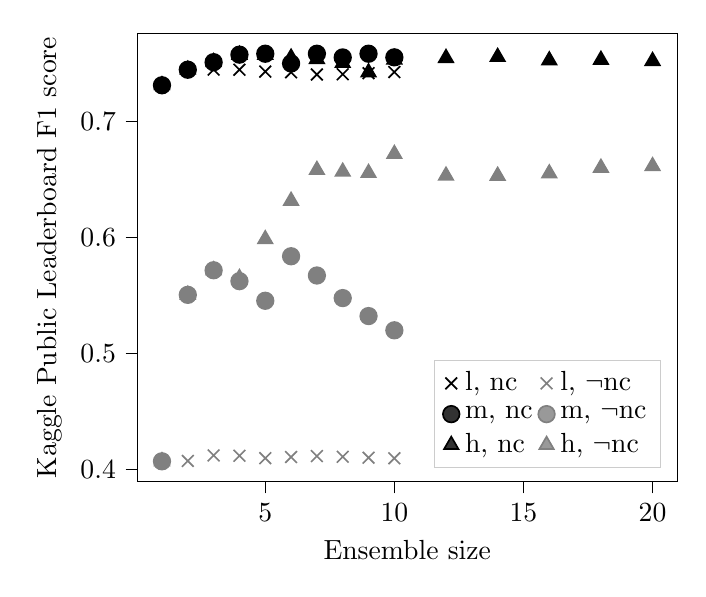
\begin{tikzpicture}

\definecolor{darkgray176}{RGB}{176,176,176}
\definecolor{gray}{RGB}{128,128,128}
\definecolor{lightgray204}{RGB}{204,204,204}

\begin{axis}[
legend cell align={left},
legend columns=2,
legend style={
  fill opacity=0.8,
  draw opacity=1,
  text opacity=1,
  at={(0.97,0.03)},
  anchor=south east,
  draw=lightgray204
},
tick align=outside,
tick pos=left,
x grid style={darkgray176},
xlabel={Ensemble size},
xmin=0.0499999999999999, xmax=20.95,
xtick style={color=black},
y grid style={darkgray176},
ylabel={Kaggle Public Leaderboard F1 score},
ymin=0.38932, ymax=0.77608,
ytick style={color=black}
]
\addplot [semithick, black, mark=x, mark size=3, mark options={solid}, only marks]
table {%
2 0.7443
3 0.7448
4 0.7447
5 0.7431
6 0.7425
7 0.7406
8 0.7408
9 0.7417
10 0.7427
};
\addlegendentry{l, nc}
\addplot [semithick, gray, mark=x, mark size=3, mark options={solid}, only marks]
table {%
1 0.4075
2 0.4072
3 0.412
4 0.4117
5 0.4096
6 0.4106
7 0.4114
8 0.4108
9 0.41
10 0.4095
};
\addlegendentry{l, $\neg$nc}
\addplot [semithick, black, mark=*, mark size=3, mark options={solid}, only marks]
table {%
1 0.7313
2 0.7447
3 0.7512
4 0.7577
5 0.7585
6 0.7501
7 0.7585
8 0.7553
9 0.7585
10 0.7554
};
\addlegendentry{m, nc}
\addplot [semithick, gray, mark=*, mark size=3, mark options={solid}, only marks]
table {%
1 0.4069
2 0.5505
3 0.5717
4 0.5623
5 0.5454
6 0.5838
7 0.5672
8 0.5477
9 0.5322
10 0.5199
};
\addlegendentry{m, $\neg$nc}
\addplot [semithick, black, mark=triangle*, mark size=3, mark options={solid}, only marks]
table {%
1 0.7313
2 0.7447
3 0.7512
4 0.7576
5 0.7576
6 0.7551
7 0.7539
8 0.7505
9 0.7424
10 0.7535
12 0.7548
14 0.7557
16 0.7528
18 0.7532
20 0.7522
};
\addlegendentry{h, nc}
\addplot [semithick, gray, mark=triangle*, mark size=3, mark options={solid}, only marks]
table {%
1 0.4069
2 0.5505
3 0.5717
4 0.565
5 0.5985
6 0.6316
7 0.6582
8 0.6567
9 0.6556
10 0.672
12 0.6533
14 0.6532
16 0.6553
18 0.6601
20 0.6615
};
\addlegendentry{h, $\neg$nc}
\end{axis}

\end{tikzpicture}
